\chapter{Method}
\label{cap:Method}

In this chapter, the method used to conduct this Master thesis will be described. The entire method is broken down into several sub processes to better structure and describe, as illustrated in  \ref{fig:Method_process}.  

\begin{figure}[H]
    \centering
    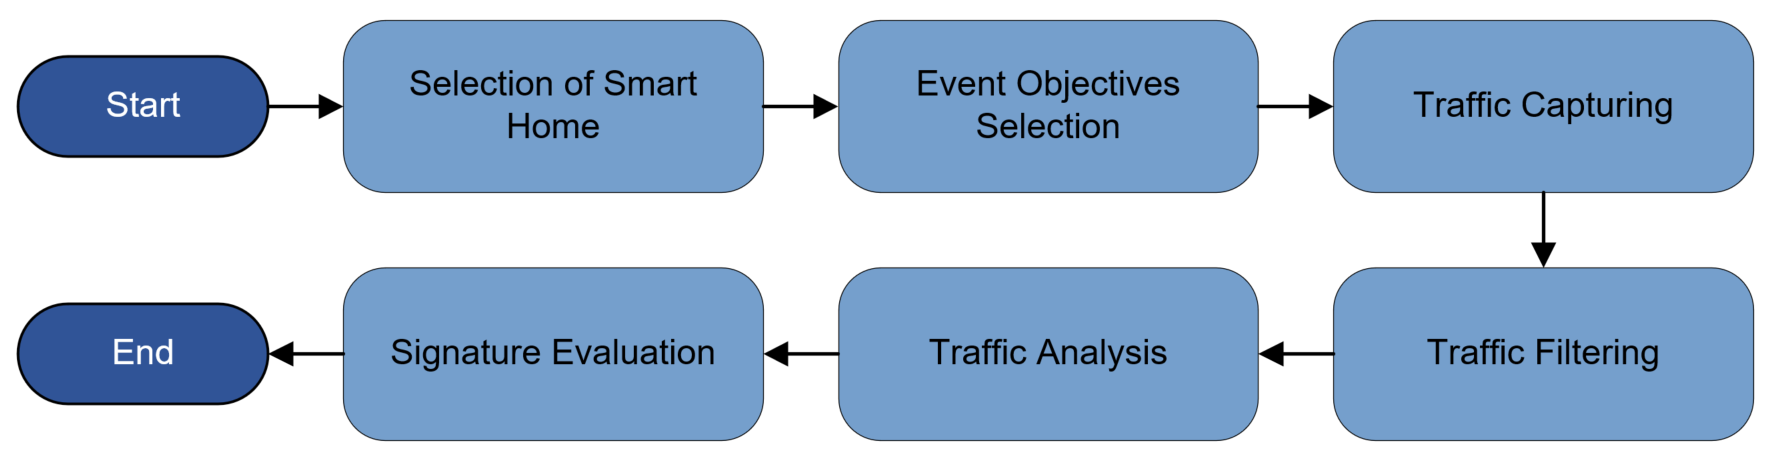
\includegraphics[width=\textwidth]{figures/Method_process.png}
    \caption{Overall Method process}
    \label{fig:Method_process}
\end{figure}



\section{Device and Environment Selection}
Due to limited financial resources it was only possible to acquire one robot vacuum cleaner. A robot vacuum cleaner survey was conducted at the start of the research, and the selection sat the requirements for the rest of the environment.  

\subsection{Selection of Robot Vacuum Cleaner Model}
Requirements for \textit{communication protocols, smart home features} and \textit{popularity} was used in the selection process. These requirements are described below.  

\begin{itemize}
    \item Communication protocol: Wi-Fi is the most wide spread communication protocol in today's smart environments \cite{robotsel1}. Eavesdropping devices and analysis tools are available for IEEE.802.11 and abstraction layers higher in the OSI model \cite{osimodel}. The selected robot vacuum cleaner therefore had to use wi-fi as a primary communication protocol.
    
    \item Smart Home Features; The robot vacuum cleaner needed several smart home features. The number features available, could increase attribution and potential information could be exposed \cite{robotsel4}.
    
    \item Popularity; The prevalence of different vendors and models will always vary, based on the number of sold and used devices. Overall usage will increase the relevance and, the scientific contribution of this research.  
\end{itemize}

Data and ratings from these three robot vacuum cleaner review sites \cite{robotsel11}\cite{robotsel12}\cite{robotsel13}, was used  as the first phase of selection. The summary of all these reviews was used to determine the most reliable robot vacuum cleaner vendors. To determine the popularity of the different vendors, downloading and ratings from Google Play was compared \cite{GooglePlay}.

\subsection{Result Selection Robot Vacuum Cleaner}

Results from the review sites is presented in Table \ref{tab:Robotreviewsites}, and shows that the two best robot vacuum cleaner vendors are, Irobot and Roborock.
\begin{table}[H]
    \centering
    \begin{subtable}[b]{0.45\linewidth}
        \centering
        \caption{Results from review-site \cite{robotsel11}}
        \begin{tabular}{|l|l|}
            \hline 
            \textbf{Vendor} & \textbf{Number on top ten} \\ \hline
            Irobot      & 3                 \\                   \hline
            Roborock    & 3                 \\                   \hline
            Neatsvor    & 0                 \\                   \hline
            Ecovacs     & 0                 \\                   \hline
            iLife       & 2                 \\                   \hline
        \end{tabular}
    \end{subtable}
    \hspace{0.5cm}
    \begin{subtable}[b]{0.45\linewidth}
        \centering
        \caption{Results from review-site \cite{robotsel12}}
        \begin{tabular}{|l|l|}
            \hline
            \textbf{Vendor}    & \textbf{Number on top ten} \\ \hline
            Irobot      & 2                 \\                   \hline
            Roborock    & 2                 \\                   \hline
            Neatsvor    & 0                 \\                   \hline
            Ecovacs     & 2                 \\                   \hline
            iLife       & 1                 \\                   \hline
        \end{tabular}
    \end{subtable}
    \begin{subtable}[b]{0.45\linewidth}
        \centering
        \caption{Results from review-site \cite{robotsel13}}
        \begin{tabular}{|l|l|}
            \hline
            \textbf{Vendor}    & \textbf{Number on top ten} \\ \hline
            Irobot      & 2                 \\                   \hline
            Roborock    & 2                 \\                   \hline
            Neatsvor    & 3                 \\                   \hline
            Ecovacs     & 1                 \\                   \hline
            iLife       & 0                 \\                   \hline
        \end{tabular}
    \end{subtable}
    \hspace{0.5cm}
    \begin{subtable}[b]{0.45\linewidth}
        \centering
        \caption{Summary of all review-sites}
        \begin{tabular}{|l|l|}
            \hline
            \textbf{Vendor}    & \textbf{Number on top ten} \\ \hline
            Irobot      & 7                 \\                   \hline
            Roborock    & 7                 \\                   \hline
            Neatsvor    & 3                 \\                   \hline
            Ecovacs     & 3                 \\                   \hline
            iLife       & 3                 \\                   \hline
        \end{tabular}
    \end{subtable}
    \caption{Robot vacuum selection review-site}
    \label{tab:Robotreviewsites}
\end{table}

Applications for different vendors' robot vacuum cleaners are presented in Table \ref{tab:VendorApplicationStat}. It is worth mentioning that the "Smart Life" application is used to control the Neatsvor vacuum cleaner, but is primarily a smart home integration application. 

\begin{table}[H]
\centering
\caption{Vendor application statistics}
\label{tab:VendorApplicationStat}
\begin{tabular}{|c|c|c|c|}
\hline
\textbf{Vendor} & \textbf{Application} & \textbf{Downloads} & \textbf{Rating} \\ \hline
Irobot          & Irobot Home          & 5 million +        & 4,0/5,0         \\ \hline
Roborock        & Roborock             & 1 million +        & 4,6/5,0         \\ \hline
Neatsvor        & Smart Life           & 10 million +       & 4,5/5,0         \\ \hline
Ecovacs         & Ecovacs Home         & 1 million +        & 2,5/5,0         \\ \hline
iLife           & iLifehome            & 50 thousand +      & NA              \\ \hline
\end{tabular}
\end{table}
Both Irobot and Roborock received seven recommendations on the review websites. This is significantly higher than the other three vendors on the list, each of which had only three representations. Additionally, both vendors were referenced in all three review sites, which strengthens their credibility. 

In the application download and rating analysis, the Neatsvor application had over 10 million downloads. However, this application is more focused on smart home integration, and the high number of downloads is likely not solely due to the robot vacuum cleaner. Meanwhile, Evacos home received a 2.5/5.0 rating, and despite having a similar number of downloads as Roborock, it fell short in the selection process. Hence, Irobot and Roborock emerged as the two most relevant vendors. In a comparison of their products, it was found that the Irobot Roomba i7 and Roborock S6 were the most suitable robots according to our requirements \cite{robotsel8} \cite{robotsel6}. 

The final comparison was conducted using \textit{bestcordlessvacuumsite.com} \cite{robotsel9}. Irobot roomba i7 and Roborck S6 have similar reviews and rating all over, and they both have a sufficient number of smart home features. The fact that the Irobot application is downloaded 5 times more than the Roborock was the decisive factor. Irobot Rommba i7 was selected, and presented in Fugure \ref{fig:irobotroombai7} 

\begin{figure}[H]
    \centering
    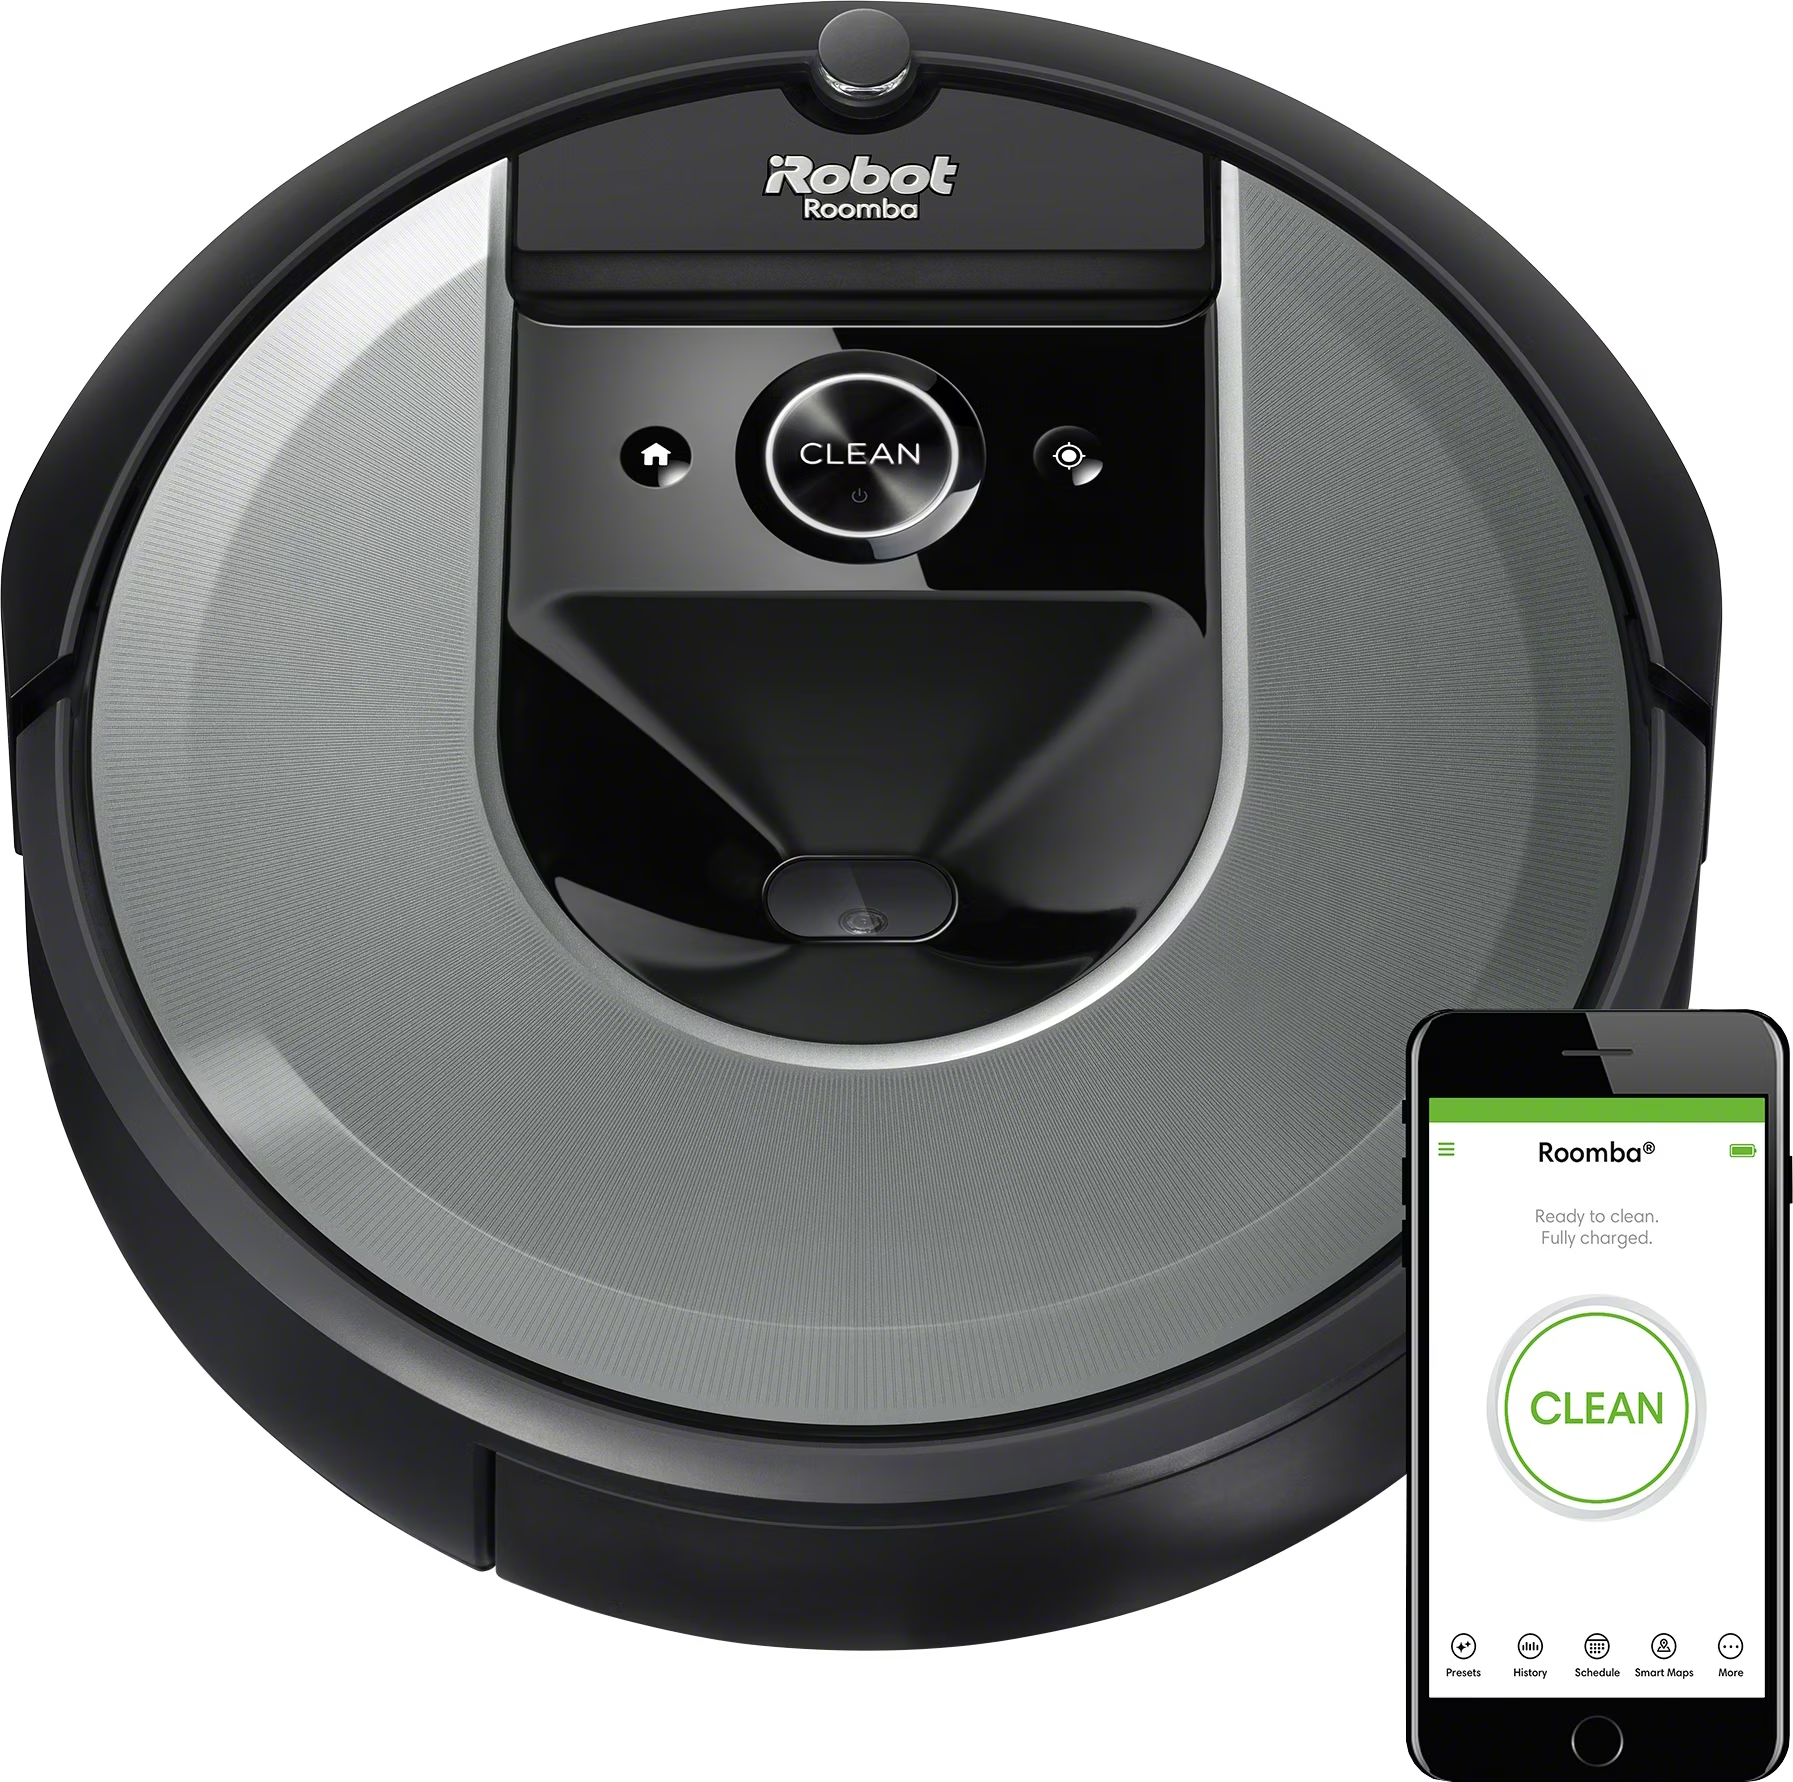
\includegraphics[width=0.5\textwidth]{figures/Irobot_picture.png}
    \caption{Irobot Roomba i7 \cite{irobotroombai7_picture}}
    \label{fig:WLAN_LAN_setup}
\end{figure}

\subsection{Environment Selection}
The rest of the research environment had to support traffic eavesdropping and analysis, of the Irobot Roomba i7. Important factors to support in research environment is listed below.

\begin{itemize}
    \item IEEE.802.11 WI-FI network
    \item Internet connection
    \item Local wired LAN
\end{itemize}

\subsubsection{Physical Environment}
To ensure the validity of the results across diverse settings, the testing was conducted in two different smart environments, now called Oslo and Drammen. These smart environments are located in two different cities. The Robot vacuum cleaner will be configured from factory defaults for each environment. Both Oslo and Drammen had independent Internet access, provided by an external Internet Service Provider (ISP). To control the duration of each test, the available test area was restricted to the one room. This decreased the duration of each test, and making the research more efficient. An illustration of Oslo and Drammen is presented in Figure \ref{fig:SmartHomeEnvironments}.

\begin{figure}[H]
    \centering
    \begin{subfigure}[b]{0.60\textwidth}
        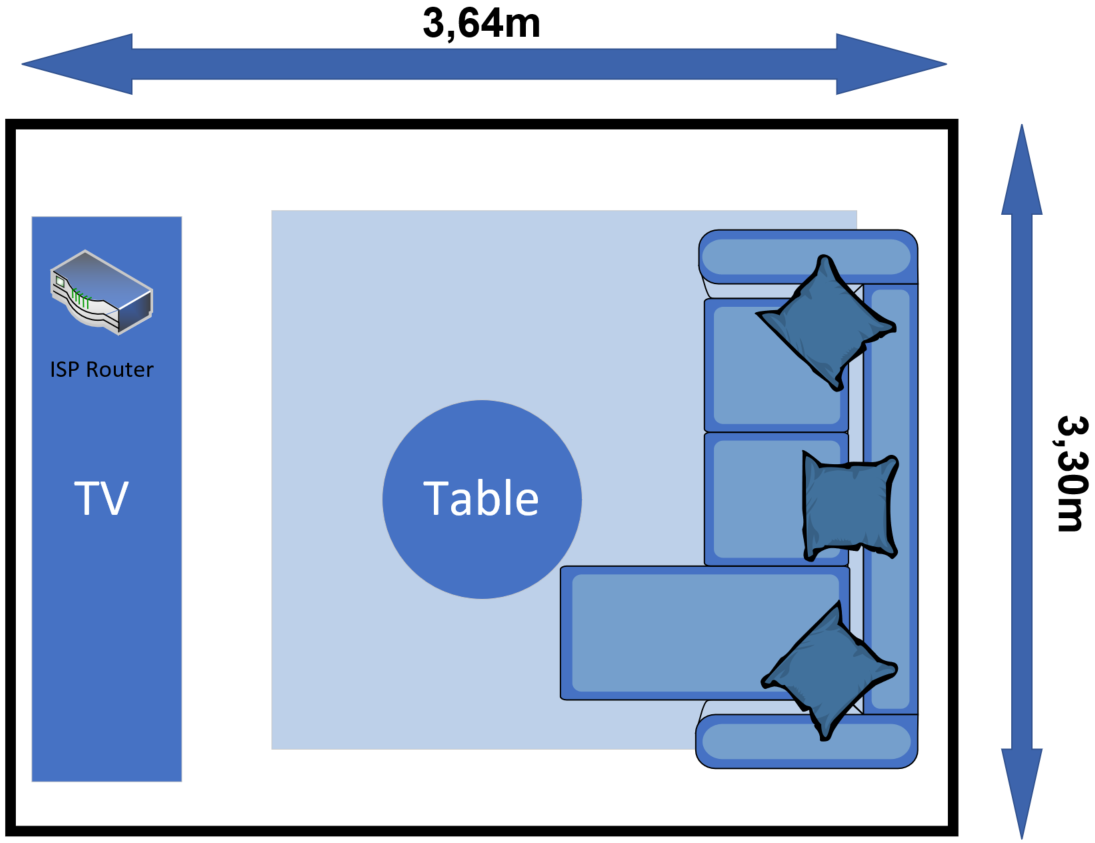
\includegraphics[width=\textwidth]{figures/Environment1.png}
        \caption{The smart home environment in Oslo}
        \label{fig:Environment1}
    \end{subfigure}
    \hfill
    \begin{subfigure}[b]{0.6\textwidth}
        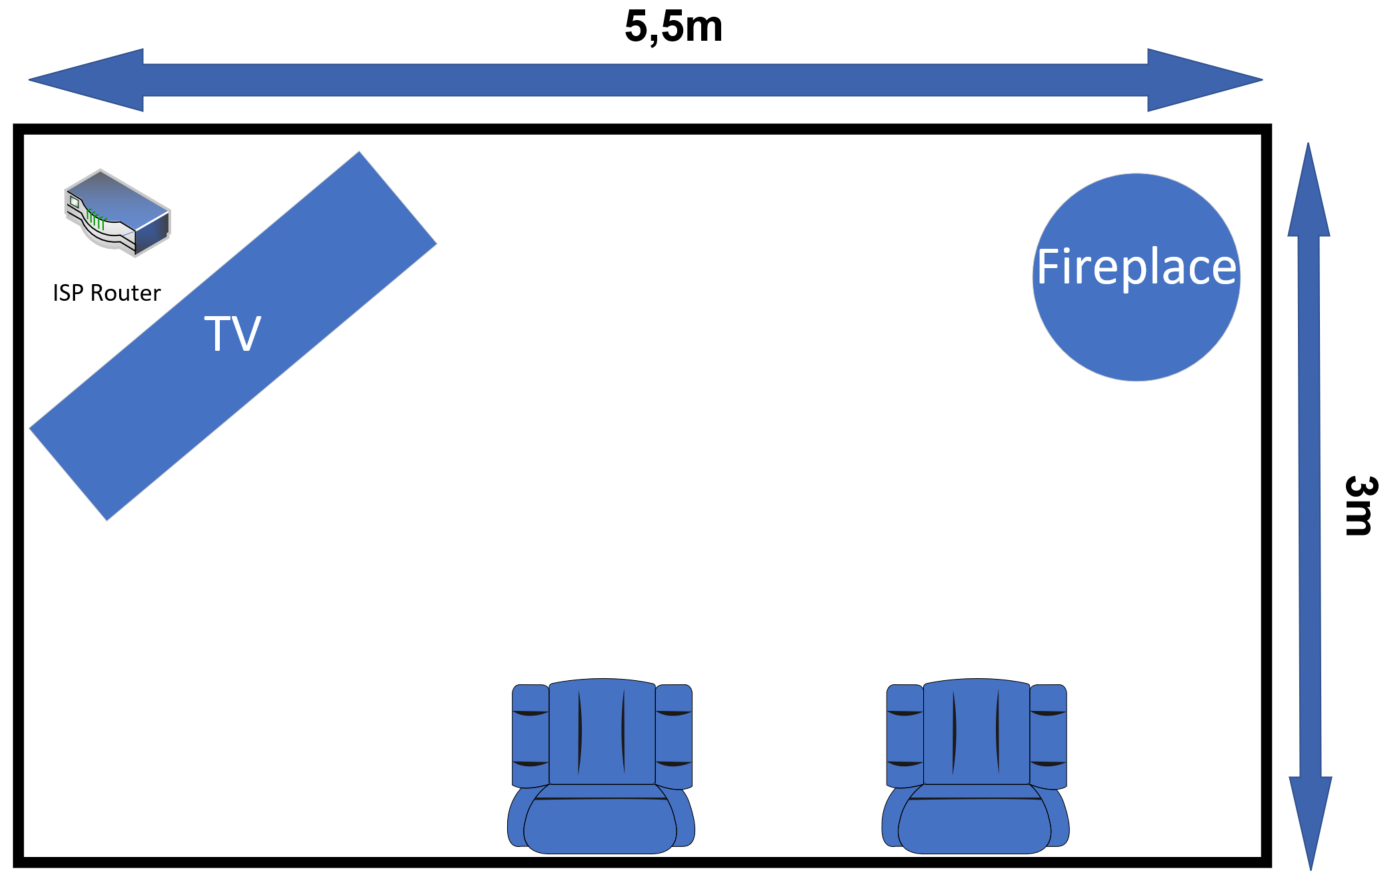
\includegraphics[width=\textwidth]{figures/Environment2.png}
        \caption{The smart home environment in Drammen}
        \label{fig:Environmet2}
    \end{subfigure}
    \caption{The smart home environments Oslo and Drammen}
    \label{fig:SmartHomeEnvironments}
\end{figure}

\subsubsection{Capturing platform}
A Raspberry PI 3b+ was chosen as the capturing platform for this research, these computers are designed to run autonomously, and has build in Ethernet and WiFi NICs. This Raspberry PI got installed with a Kali Linux operating system designed for Advanced RISC Machine (ARM) \cite{kalidownload}. Network traffic analysis and capturing tools are included in the Kali Linux distribution. During wireless capturing, the wireless NIC had to be configured in \textit{Monitor mode}. A suggested method is presented in  \cite{Kali_monitormode_guide}, used a \textit{TP-LINK TL-WN722N V2/V3}. This WiFi adapter was therefore acquired and installed on the platform. 

\subsubsection{Environment Infrastructure}
Both Oslo and Drammen had only a single ISP modem, providing both WLAN and LAN. To enable WAN interface simulation and eavesdropping, an additional Access Point (AP) and a LAN switch was installed.

The AP created a new SSID only used by the Robot vacuum cleaner, this isolated the vacuum cleaner from potential impact from other devices on the WLAN/LAN. Network Address Translation (NAT) \cite{rfc1631nat}, was translating all WiFi traffic to a singe LAN IP address. This IP address was used as the simulated WAN interface during this research.

The LAN switch was directly connected to both the AP and the ISP router, forwarding traffic towards Internet. A SPAN port was configured on the switch, monitoring traffic on the simulated WAN interface. This traffic flow got duplicated and forwarded on the port connected to the Raspberry PI. The overall network infrastructure is illustrated in Figure \ref{fig:WLAN_LAN_setup}.

\begin{figure}[H]
    \centering
    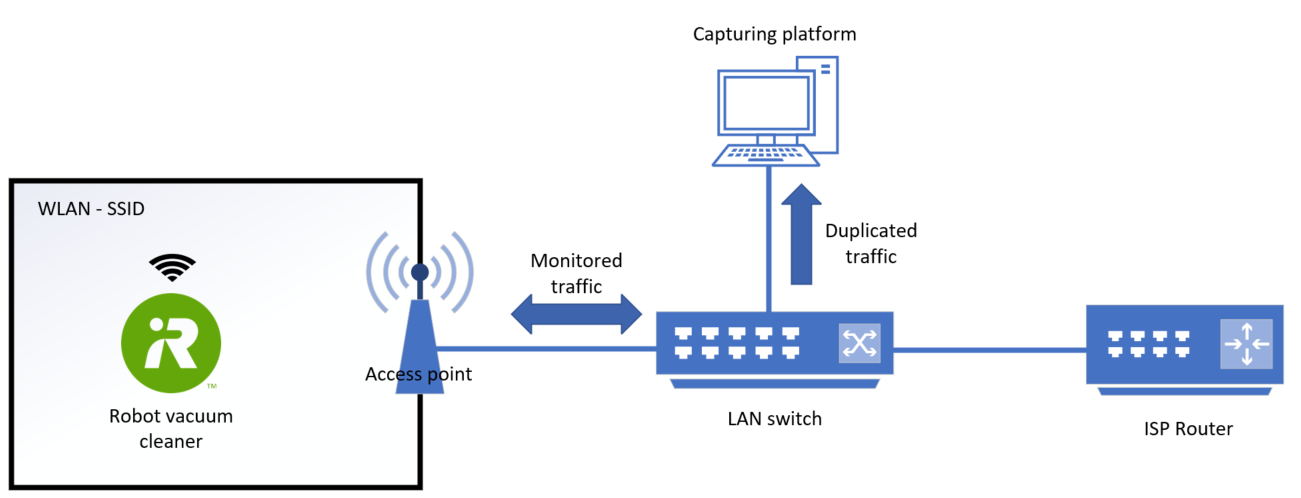
\includegraphics[width=\textwidth]{figures/WLAN_LAN_setup.png}
    \caption{Smart home infrastructure}
    \label{fig:WLAN_LAN_setup}
\end{figure}

\subsubsection{Capturing and Analysis Tools}
Whireshark is a widely used network protocol analyser, and allows network capturing and analysis in real-time. It can be used for deep header inspection in all network layers and perform basic identification of a wide range of different protocols \cite{wireshark}. This software is integrated on Kali Linux OS and is available for Windows at \cite{wireshark_download_2016}. Tshark is a subprocess of Wireshark, and can be used to capture traffic through CLI. In this process it is possible to define capturing filters which only store traffic that is interesting for the analysis phase. Tshark was therefore used to capture traffic, and the manual analysis was done with Wireshark.

\subsubsection{Device and environment specification}
This section will present the device and tool specifications used in this thesis.

\paragraph{Capturing platfrom}
Specifications are presented in \ref{tab:CapturingPlatfromSpec}

\begin{table}[H]
\centering
\caption{Capturing platform specifications}
\label{tab:CapturingPlatfromSpec}
\begin{tabular}{|ll|}
\hline
\multicolumn{2}{|c|}{\textbf{Capturing platform}}                         \\ \hline
\multicolumn{1}{|l|}{Hardware}               & Raspberry Pi 3b+           \\ \hline
\multicolumn{1}{|l|}{Software}               & Kali Linux                 \\ \hline
\multicolumn{1}{|l|}{Tshark}                 & Version                    \\ \hline
\multicolumn{1}{|l|}{External wi-fi adapter} & TP-LINK TL-WN722N V2       \\ \hline
\multicolumn{1}{|l|}{External storage}       & Micro SD card SanDisk 32GB \\ \hline
\end{tabular}
\end{table}

\paragraph{Analysis platform}
HP Elitebook with windows 11 was used as the analysis platform. It was installed with Wireshark, Tshark and Visual studio code. 

\begin{table}[H]
\centering
\caption{Analysis platform specifications}
\label{tab:AnalysisPlatfromSpec}
\begin{tabular}{|ll|}
\hline
\multicolumn{2}{|c|}{\textbf{Analysis platform}}      \\ \hline
\multicolumn{1}{|l|}{Hardware}  & HP Elitebook        \\ \hline
\multicolumn{1}{|l|}{Software}  & Windows 11          \\ \hline
\multicolumn{1}{|l|}{Wireshark} & 4.0.2               \\ \hline
\multicolumn{1}{|l|}{VS code}   & 1.77.3 (user setup) \\ \hline
\end{tabular}
\end{table}

\paragraph{Access point}
TP-Link Archer MR200 was acquired, specifications listed in Table \ref{tab:AccessPointSpec} 

\begin{table}[H]
\centering
\caption{Access point specifications}
\label{tab:AccessPointSpec}
\begin{tabular}{|ll|}
\hline
\multicolumn{2}{|c|}{\textbf{Access Point}}                        \\ \hline
\multicolumn{1}{|l|}{Hardware} & TP-Link archer MR200(EU) ver:5.30 \\ \hline
\multicolumn{1}{|l|}{Software} & version                           \\ \hline
\end{tabular}
\end{table}

\paragraph{LAN switch}
A Cisco Catalyst 2960 series switch was used, this due to the support for SPAN port configuration. Specifications presented in Table \ref{tab:LanSwitchSpec}.

\begin{table}[H]
\centering
\caption{LAN Switch specifications}
\label{tab:LanSwitchSpec}
\begin{tabular}{|ll|}
\hline
\multicolumn{2}{|c|}{\textbf{LAN Switch}}                           \\ \hline
\multicolumn{1}{|l|}{Hardware} & Cisco Catalyst 2960 series, 8 port \\ \hline
\multicolumn{1}{|l|}{Software} & ISO 12.2(35)SE5                    \\ \hline
\end{tabular}
\end{table}


\paragraph{Network architecture}
Oslo and Drammen will have the same network infrastructure, except the local ISP modem. This architecture in presented in Figure \ref{fig:SmartHomeSetup}. 

\begin{figure}[H]
    \centering
    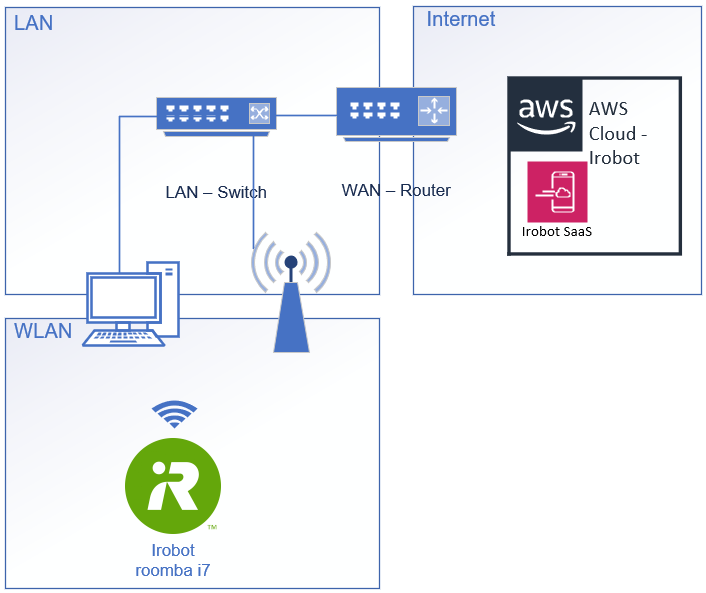
\includegraphics[width=0.8\textwidth]{figures/SmartHomeSetup.png}
    \caption{SmartHomeSetup}
    \label{fig:SmartHomeSetup}
\end{figure}






\section{Traffic Capturing}
This section will describe how the capturing tools are used, and how the overall capturing process is executed. Capturing of WLAN and WAN traffic was done simultaneously of the Raspberry PI, creating a foundation for WAN and WLAN event comparison. 

\subsection{Captuing Tools}
Two Tshark processes was executed simultaneously on the Raspberry PI, one instance captured WAN traffic on the Ethernet port (eth0) and the other capturing WLAN traffic on the WiFi adapter interface (wlan1). Both instanced had a capturing filter argument, capturing only traffic relevant for the analysis phase. Syntax for Tshark filter is described on \cite{tshark_filter}. The Tshark arguments used in these captures, was interface specification \textit{-i}, traffic filter \textit{-f} and output file name \textit{-w}. Filtering was based on the Irobot Roomba's WiFi MAC address for WLAN, and the simulated WAN IP-address for LAN. Due to local user restrictions the Tshark commands was executed in sudo mode. Tshark filter syntax as well as, WLAN and LAN specific syntax are listed below. 

\begin{itemize}
    \item \textbf{tshark [ -i <capture interface> ] [ -f <capture filter> ] [ -w <outfile> ]}
    \item \textbf{sudo tshark -i wlan1 -f 'eth.host 'MAC address' -w output.pcap}
    \item \textbf{sudo tshark -i eth0 -f 'ip.host "WAN address' -w output.pcap}
\end{itemize}

\subsection{Capturing Process}
A fixed capturing process was used the entire research, this created the best foundation for event comparison. The entire capturing process is illustrated with a flow diagram in Figure \ref{fig:captuingprocess}. First both WLAN and LAN Tshark capturing was started. While these captures ran, events was triggered according to a test matrix. The file size of the output file was continuously check, if the file size exceeded 500 Mb it would decrease Wireshark's ability to analyze the capture \cite{wireshark}. Both capturing processes was then restarted with a new output file. When all events had been triggered, the capturing was stopped, and files were extracted to an Windows machine for further analysis, through WinSCP \cite{winscp2023}.
  
\begin{figure}[H]
    \centering
    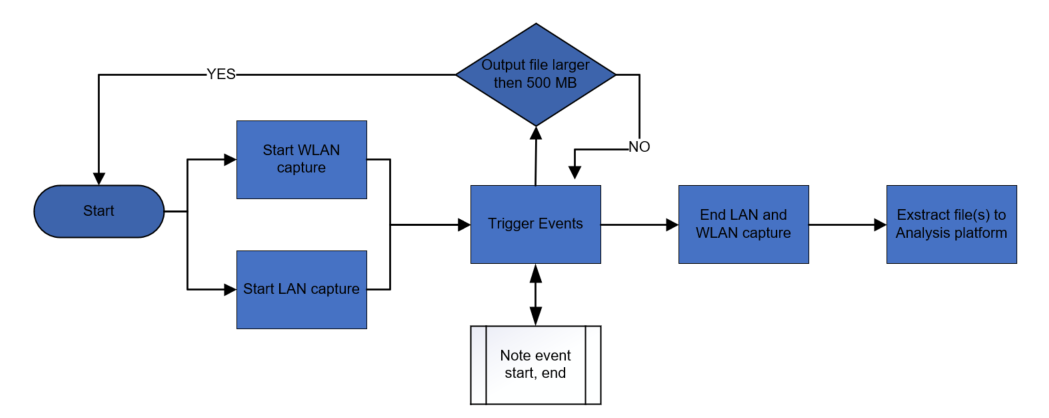
\includegraphics[width=\textwidth]{figures/Event triggering process.png}
    \caption{Capturing process}
    \label{fig:captuingprocess}
\end{figure}

\subsection{Event Selection}
This section will present the different smart features on Irobot Roomba i7, selected as event objectives in this thesis. First a \textit{Standby event} was conducted, this was done one time in Oslo and  was used to create base filter for the analysis phase. The event objectives are \textit{Scheduled cleaning, Automated cleaning, Application triggered cleaning, Physical triggered cleaning, Application start} and \textit{Bin remove}. These events was triggered ten times for each of the environments Oslo and Drammen. This generated 20 captures of each event and was decided to be a sufficient number of captures, to determine patterns. All cleaning events used a customized cleaning area which defined the entire smart map of the environment.   

\subsubsection{Standby Traffic}
This test was executed to identify network traffic generated by the robot vacuum cleaner in a standby mode. No human interaction was done during the event. All identified traffic pattern in this capture, is therefore irrelevant for the event objectives. The event flow is listed below. 

 \begin{enumerate}
         \item Start captuing of LAN and WLAN traffic
         \item Wait 14 days without any human interaction
         \item Stop capturing
\end{enumerate}

\subsubsection{Scheduled Cleaning}
Scheduled cleaning can be configured through the smart phone application. Users can schedule a cleaning by specifying area in the smart environment and time which the cleaning should start. The event flow is presented below, and was used for triggering all cleaning events in this thesis. 

\begin{enumerate}
  \item Trigger cleaning event
  \item Note when "finish" notification is received
  \item Stop capturing
\end{enumerate}


\subsubsection{Automated Cleaning}
Irobot has features to integrate other services as trigger for events. This includes IFTTT location tracker \cite{ifttt}, Agust smart lock system, ecobee termotat system, My Leviton smart home integration and MyQ garage system \cite{irobot}. In this research the IFTTT location system was used as event trigger. Cleaning was then triggered when the user's phone was N meters away from home. This event had the same flow as scheduled cleaning event. 

\subsubsection{Application Triggered Cleaning}
Users can trigger cleaning events manually through the application. This cleaning event was triggered when the user manually started the application and pressed the customized cleaning option. The event had the same flow as scheduled cleaning event.


\subsubsection{Physical Triggered Cleaning}
The Irobot roomba i7 has a physical cleaning button on top of the vacuum cleaner. A "clean all" event is triggered when this button is pressed. This event had the same flow as the other cleaning events.

\subsubsection{Application Start}
When the application is started, a dashboard is displayed. Users can then interact with the vacuum cleaner. The event flow of this event is listed below. 

 \begin{enumerate}
                                    \item Note time
                                    \item Open the application on the smart phone
                                    \item Wait for some time
                                    \item Close application
                                    \item Note time
 \end{enumerate}


\subsubsection{Bin Remove}
The Irobot roomba i7 has it own bin where dust is collected during clean. This can be removed to empty. The event flow is listed below. 

\begin{enumerate}
                                    \item Note time
                                    \item Remove the bin
                                    \item Wait  more then 30 seconds
                                    \item Insert the bin
                                    \item Note time
 \end{enumerate}


\section{Traffic Filtering}
The traffic filtering work flow is presented in Figure \ref{fig:TrafficProcessingProcess}. This process is based in the \textit{Standby event}, manual analysis in Wireshark was used to identify irrelevant protocols and traffic. The findings was added to the base filter in a iterative process. This excluded more and more traffic, reveling less prominent traffic to be identified.  

\begin{figure}[H]
    \centering
    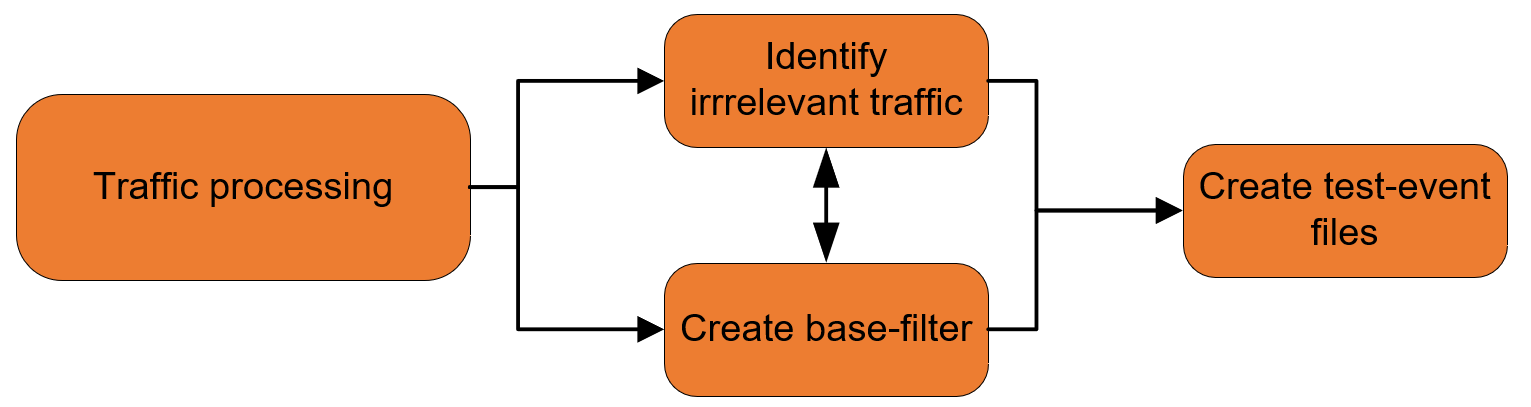
\includegraphics[width=\textwidth]{figures/TrafficProcessingProcess.png}
    \caption{Traffic processing}
    \label{fig:TrafficProcessingProcess}
\end{figure}

The Wireshark base filter was constructed as a logically equation, including AND, OR and NOT operators. Each of the irrelevant traffic flows identified in the iterative filtering process was added into the equation. The last step of the filtering process was to extract .pcap files, only including one event. This was done with wireshark time filtering, based in the overall test matrix. Wireshark time filter applied to the original capture files is:
\textbf{(frame.len >= " Month day, start-time") \&\& (frame.len <= "Month day, end-time")}


\section{Traffic Analysis}
The traffic analysis workflow is presented in Figure \ref{fig:TrafficAnalysisProcess}, and included three subprocesses \textit{protocol and event relation, Traffic sequence identification} and \textit{Overall event characteristics}. Results from all these subprcesses was used to create event signatures. All signatures was then compared to identify if they overlapped with other events. 

\begin{figure}[H]
    \centering
    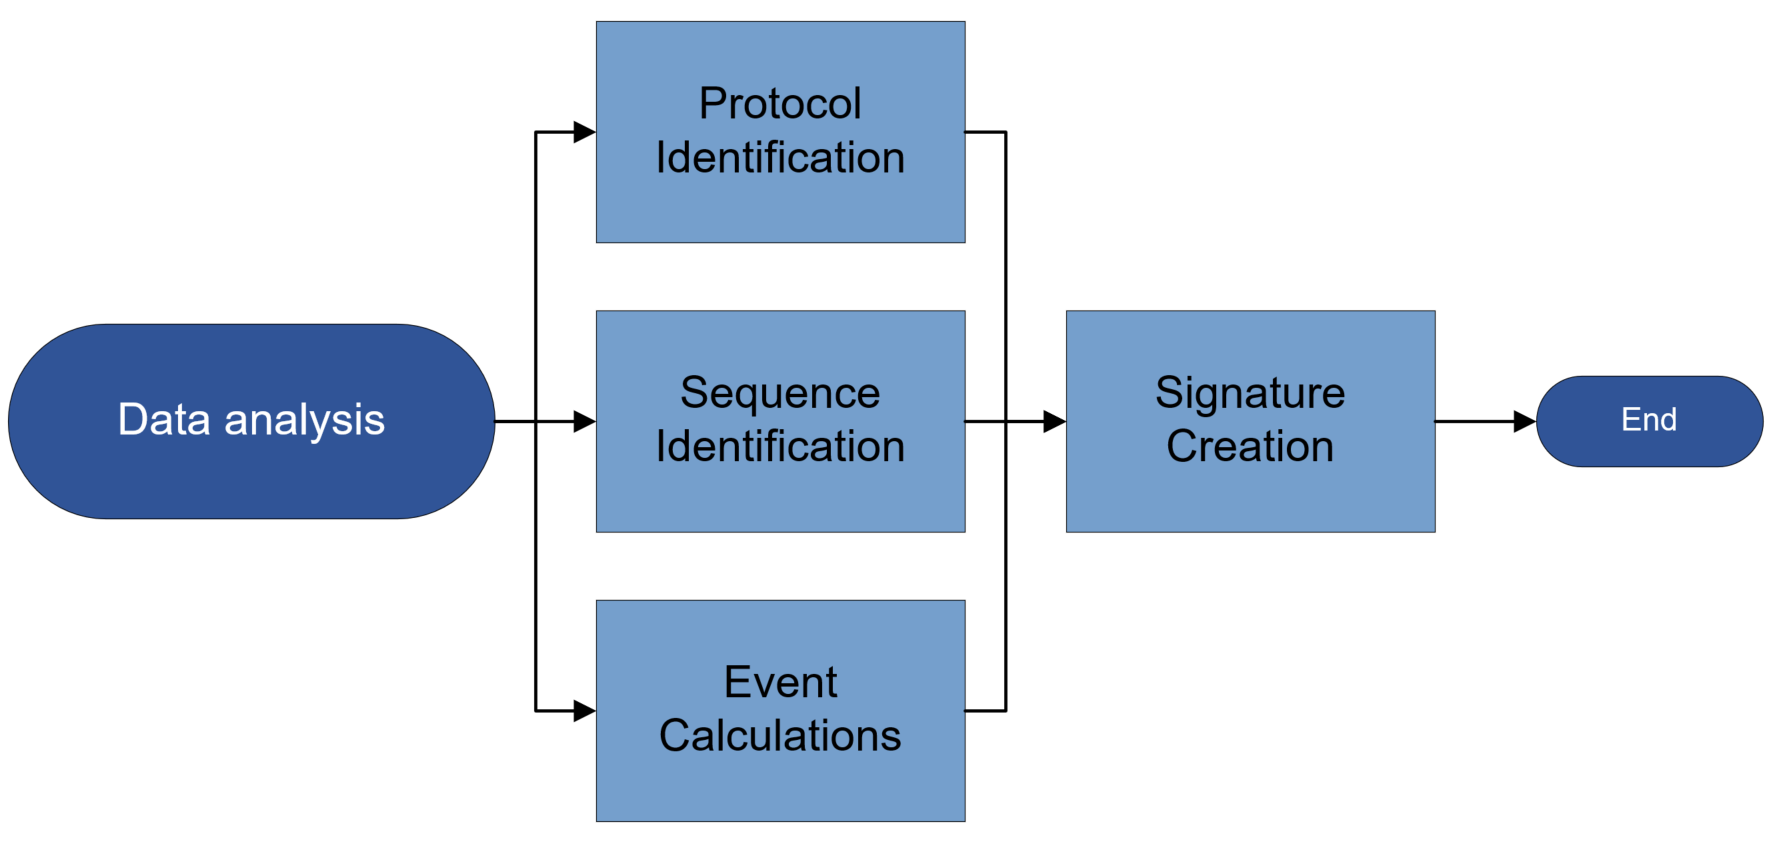
\includegraphics[width=\textwidth]{figures/TrafficAnalysisProcess.png}
    \caption{Traffic Analysis Process}
    \label{fig:TrafficAnalysisProcess}
\end{figure}

\subsection{Protocol Event Relation}
Wiresharks was used to analyze protocol and event relations. If protocols occur of a specific event it might be a good indication to use in the event signature. Protocol statistic tools in Wireshark was used for this identification, an example of this tool is presented in Figure \ref{fig:wiresharkprotocolstatistictools}. Further a filter only including the interesting protocols was applied, making it easier to identify interesting  protocol attributes.

\begin{figure}[H]
    \centering
    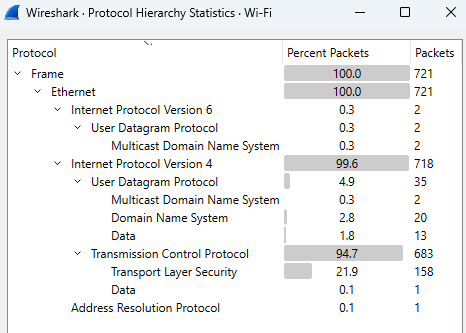
\includegraphics[width=0.8\textwidth]{figures/wireshark_protocol_hirarcy.png}
    \caption{Wireshark protocol statistic tool}
    \label{fig:wiresharkprotocolstatistictools}
\end{figure}

\subsection{Traffic Sequence}
Traffic sequence analysis used the same attributes as Trimananda et al.  \cite{pingpong_trimananda2020packet}, but not the proposed ML algorithm. Packet length sequences was extracted with the use of python scripting including pyshark library, and analyzed manually by humans. This analysis also included the sequence of protocols, enabling signatures based on more then just packet lengths as attributes. Traffic flow directions was also taken in to account during this process. This included the traffic flows listed below. 
  
\begin{itemize}
    \item Traffic both directions.
    \item Traffic with vacuum cleaner as source.
    \item Traffic with vacuum cleaner as destination.
\end{itemize}

\subsection{Overall Event Characteristics}
Overall characteristics of each event file was analyzed, and used to determine if the number of 20 events was sufficient. Extracted information about \textit{number of packets, total bytes sent} and \textit{protocols}, was used in this process. Standard deviation of these data indicated the consistency of each event objective. 

\subsection{Event Signatures}
Results of the three sub processes was used to propose an event signature. Attributes in the different signatures was implemented as search conditions in a python function. A separate function was created for each event signature, returning a confident variable to the main function. This enables the detection algorithm to add new signatures to increase the detection confidence of an event. All these functions followed the same logical flow as presented in Figure \ref{fig:Sudo_code_signature_function}

\begin{figure}[H]
    \centering
    \caption{Sudo code for signature function}
    \label{fig:Sudo_code_signature_function}
    \begin{lstlisting}[numbers=left]
     def Identify_event(event_file, event_confidence_variable):
         event_siganture = ['siganture']
         if event_signature is in eventfile:
             event_confident_variabel =+ level_of_confidece
         else
             None
         return event_confodence_variabel
    \end{lstlisting}
\end{figure}

\section{Signature Detection and Evaluation}
All signature functions was integrated in a main python script. This script imports selected pcap files and run through all the signature functions. True positive and False positive detection increases the confident variable for each event. A comparison of the confidence variables are executed at the end, to determine which event is most likely to have been triggered. The main function follows the logic presented in Figure \ref{fig:Sudo_code_event_detection_alg}.

\begin{figure}[H]
    \centering
    \caption{Sudo code event detection algorithm}
    \label{fig:Sudo_code_event_detection_alg}
    \begin{lstlisting}[numbers=left]
         Main()
              #import event pcap file
              Capture = import(Event_file_x)
              #Run detection functions, and create confidence variables
              #eventX_confident_variable = eX_cv  
              e1_cv = identify_event1(Capture, event1_confodence_variable)
              e2_cv = identify_event2(Capture, event1_confodence_variable)
              e3_cv = identify_event3(Capture, event1_confodence_variable)
              e4_cv = identify_event4(Capture, event1_confodence_variable)
              e5_cv = identify_event5(Capture, event1_confodence_variable)
              e6_cv = identify_event6(Capture, event1_confodence_variable)
              #comapre event_confident_variables highest is event
              confident_variables = [list of all variables]
              for event in range(1,6)
                   if confidentvariabels[event] is larger then last number
                       largest = confidentvariabels[event]  
    \end{lstlisting}
\end{figure}

